\section{Preliminary Definitions}
\label{sec:background}

\subsection{Domain-Specific Languages in a nutshell}

%As aforementioned, a DSL is a set of language constructs each of which represents certain abstraction in a particular domain. In the general case, a DSL offers an editor that provides the capabilities needed to write programs (textually or graphically) by using the language constructs. Once a the program is written, it can be used as part of the implementation artifacts of a system under construction. 


\subsubsection{Specification:} Like general purpose languages (GPLs), DSLs are defined in terms of syntax and semantics \cite{Harel:2004b}. Hence, the specification of a DSL is a tuple $<syn,sem,M_{syn\leftarrow sem}>$ \cite{Combemale:2013}. The parameter $syn$ (the \textit{\textbf{syn}tax}) refers to the structure of the DSL and specifies each language construct in terms of its name and the relationships it has with other language constructs. In turn, the parameter $sem$ (the \textit{\textbf{sem}antics}) refers to the meaning of the language constructs. This meaning corresponds to the dynamic behavior that establishes the manner in which language constructs are manipulated at runtime. Finally, the parameter $M_{syn\leftarrow sem}$ refers to the mapping between the language constructs and the semantics. 


%The \textit{concrete syntax} refers to the association of the language constructs to the set of symbols (either graphical or textual) offered by the editor.
\vspace{-2mm}
\subsubsection{Technological space:} Currently, there are diverse techniques available for the implementation of syntax and semantics of DSLs \cite{Mernik:2005b}. Language designers can, for example, choose between using context-free grammars or metamodels as specification formalism for syntax. Similarly, there are at least three methods for expressing semantics: operationally, denotationally, and axiomatically \cite{Mosses:2001}. In this paper we are interested on DSLs which syntax is specified by means of metamodels and semantics is specified operationally as a set methods (a.k.a, \textit{domain-specific actions} \cite{Combemale:2013}). Each language construct is specified by means a metaclass and the relationship between language constructs are specified as references between metaclasses. In turn, domain-specific actions are specified as java-like methods that are allocated in each metaclass.

\vspace{-2mm}
\subsubsection{Implementation:} In order to implement a DSL, language designers need a tool set that offer capabilities to specify a DSL according to the selected technological space. This kind of tool sets are provided by language workbenches (such as Eclipse Modeling Framework or MetaEdit+) that provide meta-languages for where syntax and semantics can be expressed. The ideas presented in this paper are implemented in an Eclipse-based language workbench. In particular, metamodels are specified in the Ecore language whereas domain-specific actions are specified as methods in Xtend programming language\footnote{\url{http://www.eclipse.org/xtend/}}. The mapping between metaclasses and domain-specific actions is specified by using the notion of aspect introduced by the Kermeta 3\footnote{\url{https://github.com/diverse-project/k3/wiki/Defining-aspects-in-Kermeta-3}} and Melange\footnote{\url{http://melange-lang.org/}} as explained in \cite{degueule:2015}. 

\subsection{On the notions of \textit{commonalities} and \textit{potential reuse} in DSLs}

By definition, DSLs are scoped to specific domains so they provide restricted set of language constructs. As a result, there is a proliferation of many DSLs in the literature each of which is useful in certain application contexts \cite{Mernik:2005b}. Although many of those existing DSLs are completely different and tackle independent domains; there are related DSLs with overlapping domains \cite[p. 60-61]{voelter:2013}. That is, they share certain language constructs i.e., they have \textbf{commonalities} between them. If two DSLs have commonalities and they are specified in the same technological space and using compatible language workbenches, then there is \textbf{potential reuse} since the specification of those shared constructs can be specified once and reused in the two DSLs \cite[p. 60-61]{voelter:2013}.

Naturally, commonalities can be found not only at the level of the syntax but also at the level of the semantics. For the technological space discussed in this paper, syntactic commonalities appear where DSLs share some metaclasses and semantic commonalities appear where DSLs share some domain-specific actions.

\vspace{-1mm}
\subsubsection{Example:} Let us now introduce a toy example to illustrate the concepts introduced so far. Consider the following set of three DSLs:

\begin{itemize}
\item \textbf{Finite State Machines (FSM):} FSM is a DSL for expressing simple state machines with states and transitions between the states. Each state has an associated action that allow the modification of some data (variables) in a given execution context. In turn, each transition may define a guard (evaluated in the execution context) that expresses the condition(s) under the transition can be fired.

\vspace{2mm}
\item \textbf{Logo:} Logo is a DSL for expressing movements of the classical Logo turtle used in elementary schools for teaching the first foundations of programming. This DSL offers the constructs for moving a turtle forward and backward, as well for rotating the turtle at the left or at the right. In addition, the DSL offers simple arithmetic expressions for indicating the distance/angles the must should move/rotate. 

\vspace{2mm}
\item \textbf{Flowchart:} Flowchart is a DSL for expressing simple flow diagrams. Each flow is a sequence of nodes and arcs between them. An arc can be either an action or a decision. An action is a set of instructions that modify some variables in the execution context. A decision is a bifurcation point where depending on a given condition the flow goes from a direction or another. 
\end{itemize}

These DSLs are essentially different. Each of them is focus on a particular domain and offers different language constructs. However, there are syntactic and semantic commonalities that are illustrated in Figure \ref{fig:domains}. All the thee DSLs offer some expressions for modifying variables. In the case of FSM these actions are needed the specification of the actions in the states; in the case of Logo expressions are needed to specity the movement and rotation parameters; and in the case of flowchart expressions are needed to specify the body of actions. In addition, both FSM and Flowchart rely on a constraints language. The former for expressing guards in the transitions and the later for expressing guards of the decisions.

Note that each DSL is specified in terms of a set of metaclasses (top of the figure), and a set of aspects (bottom of the figure) that weave some domain-specific actions to the metaclasses. In the case of this example, the semantics of the metaclasses expression and constraints are also shared. That means that the semantics are the same. 

\begin{figure}
\centering
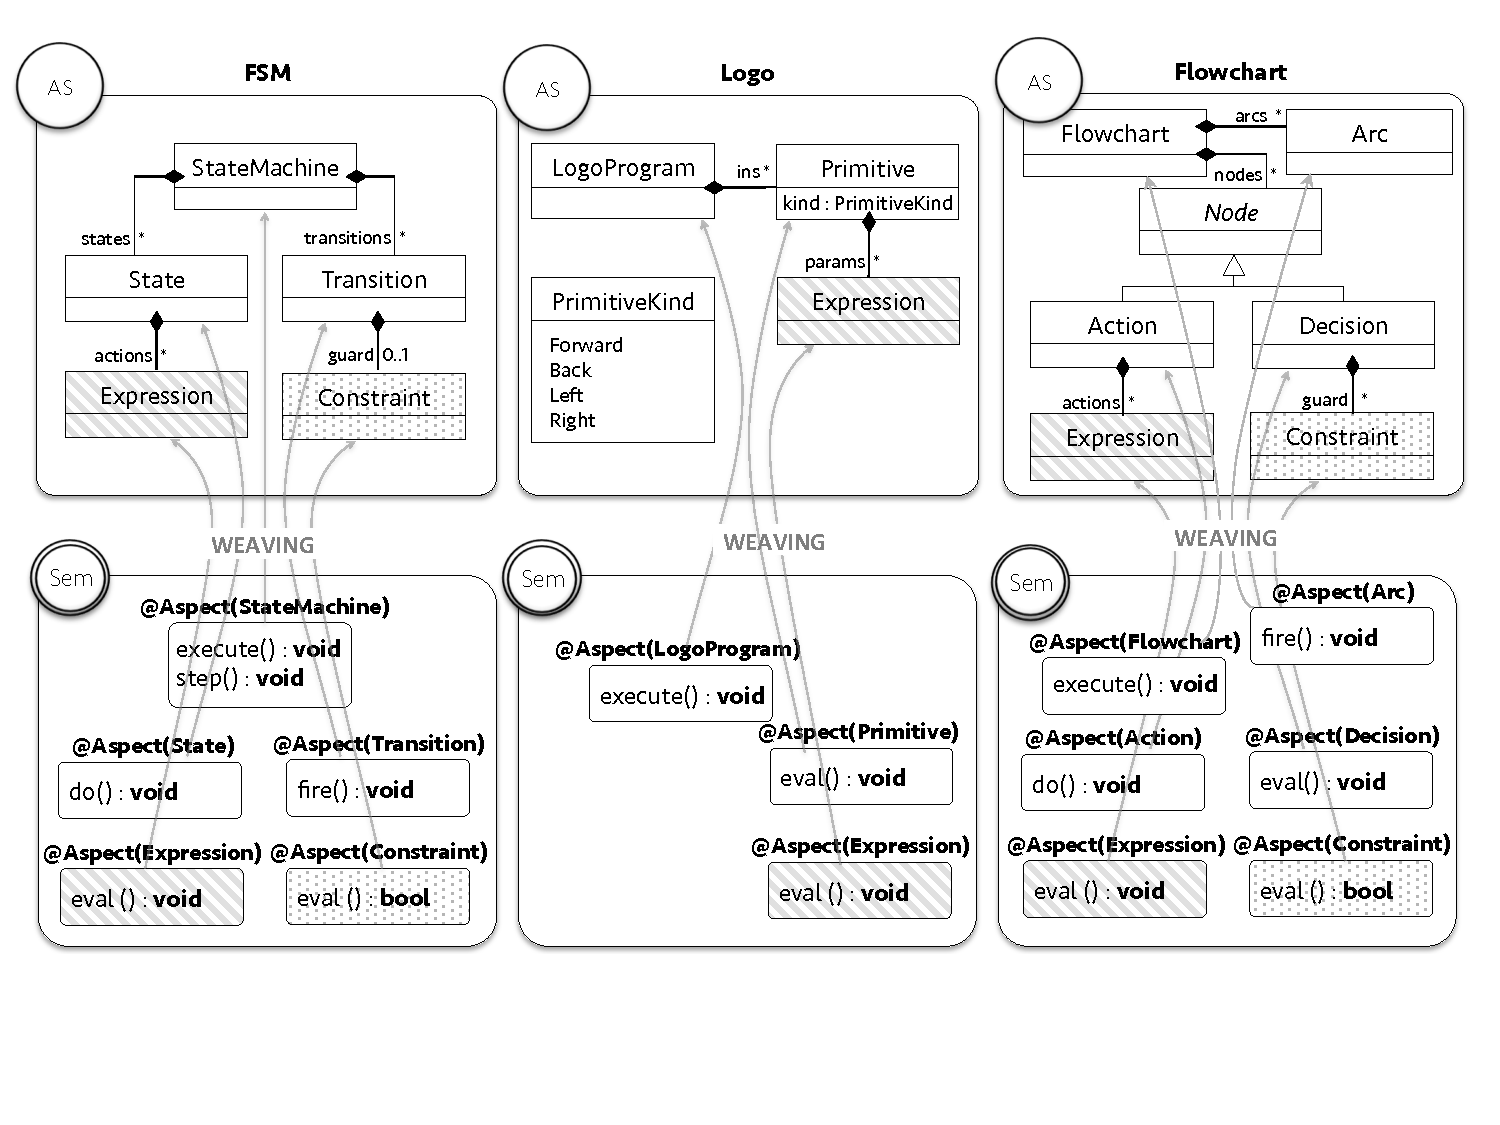
\includegraphics[width=1\linewidth]{images/domains-fig.pdf}
\caption{Commonalities between domains and potential reuse}
\label{fig:domains}
\end{figure}

%Commonalities can be found between two ore more DSLs of the input set. That is, we can find metaclasses and domain specific actions that are shared by more than two DSLs. Hence, intersections should be searched among all the possible combinations of the DSLs in the input set. Once those functions are defined and implemented, the second phase is to use them in order to find the intersections among the DSLs of the input set. 

\vspace{-3mm}
\subsubsection{Semantical variability:} It is worth to mention that the fact that two metaclasses are shared does not imply that all their domain specific actions are the same. We refer to that phenomenon as \textit{semantical variability}. There are two constructs that share the syntax but that differ in their semantics. In such case, there is potential reuse at the level of the syntax since the metaclass can be defined once and reused in the DSLs but the semantics should be defined differently for each DSLs. 

%there are three DSLs DSLs that are totally independent. That means that they do not share any of their language constructs, and consequently, there is not potential reuse between them. Differently, the two DSLs shown at the right of the figure have overlapping domains. That means that there are a subset of language that are \large\textbf{``equal'' }\normalsize in both DSLs. Note that if two language constructs are the same, we can assume that their specifications are equal and can be reused instead of being replicated.




%Moreover, there are set of DSLs for which the domains can be hierarchically organized \cite[p. 60-61]{voelter:2013}.

%\subsection{Equivalence between language constructs}

%So far, we have based the notion of potential reuse in DSLs on the commonalities existing in a set of DSLs. Nevertheless, this assumption supposes that we are able to compare two language constructs in order to know if they are equivalent. So, now we need to define this \textit{equivalence} relationship. In particular, the comparison of two language constructs relies on two dimensions: (1) comparison of the meta-classes in the abstract syntax; and (2) comparison of the domain-specific actions in the semantics.

